%%%%%%%%%%%%%%%%%%%%%%%%%%%%%%%%%%%%%%%%%%%%%%%%%%%%%%%%%%%%%%%%%%%%%%%%%%%%
%
%  tutorial.tex
%
%  Introductory tutorial for new users of Ludwig. 
%
%  Edinburgh Soft Matter and Statistical Physics Group and
%  Edinburgh Parallel Computing Centre and
%  Department of Physics, University of Strathclyde
%
%  Contributing authors:
%  Oliver Henrich (oliver.henrich@strath.ac.uk)
%  Fraser Mackay (s1026487@sms.ed.ac.uk)
%
%  (c) 2008-2017 The University of Edinburgh
%
%%%%%%%%%%%%%%%%%%%%%%%%%%%%%%%%%%%%%%%%%%%%%%%%%%%%%%%%%%%%%%%%%%%%%%%%%%%%

\documentclass[11pt,twoside,a4paper]{article}

\usepackage{amsmath}
\usepackage{moreverb}
\usepackage{lscape}
\usepackage{epic}
\usepackage[pdftex]{graphicx}
\usepackage{bm}
\usepackage{hyperref}
\usepackage{color}
\usepackage{listings}
\usepackage{mathtools}
\usepackage{enumerate}
\usepackage{float}
\usepackage{hyperref}
\graphicspath{{./tutorialFigs/}}

\usepackage{geometry}
 \geometry{
 a4paper,
 left=3.1cm,
 right=3.1cm,
 top=2.25cm,
 bottom=2.25cm 
}

\setlength{\parindent}{0pt}
\setlength{\parskip}{\smallskipamount}

\newcommand{\inputkey}[1]{\framebox{\textbf{\texttt{#1}}}}
\newcommand{\e}[1]{\cdot10^{#1}}
\newcommand{\beq}{\begin{equation}}
\newcommand{\eeq}{\end{equation}}
\newcommand{\beqa}{\begin{eqnarray}}
\newcommand{\eeqa}{\end{eqnarray}}
\newcommand{\com}[1]{\textcolor{red}{#1}}
\newcommand{\plag}[1]{\textcolor{green}{#1}}
\newcommand{\cur}[1]{{\textit{#1}}}

\definecolor{terminalcolour}{gray}{0.96}

\lstdefinestyle{terminalverbatim}{
  basicstyle=\small\ttfamily,
  columns=flexible,
  backgroundcolor=\color{terminalcolour},
  xleftmargin=0pt
}


\begin{document}


\setcounter{page}{1}

% We're not including the table of contents just at the moment
%\tableofcontents

\newpage
\lstset{style=terminalverbatim}

\setcounter{page}{1}

% These redefinitions are just compressing the spacing a little.

\makeatletter
\renewcommand*{\section}{%
\@startsection {section}{1}{\z@}%
  {-1.75ex \@plus -0.5ex \@minus -.1ex}%
  {1.15ex \@plus.1ex}%
  {\normalfont\Large\bfseries}%
}
\renewcommand*{\subsection}{%
\@startsection {subsection}{2}{\z@}%
  {-1.75ex \@plus -0.5ex \@minus -.1ex}%
  {1.15ex \@plus.1ex}%
  {\normalfont\large\bfseries}%
}
\renewcommand*{\subsubsection}{%
\@startsection {subsubsection}{1}{\z@}%
  {-1.75ex \@plus -0.5ex \@minus -.1ex}%
  {1.15ex \@plus.1ex}%
  {\normalfont\normalsize\bfseries}%
}

% Table of Contents
\pagenumbering{roman}
\title{Ludwig User Tutorial}
\author{Fraser Mackay and Oliver Henrich}
\maketitle 
\tableofcontents
\clearpage

% Sections
\pagenumbering{arabic}

\section{Introduction}

This tutorial document takes new users of the \texttt{Ludwig} code through the process of how to obtain 
and build the code before outlining some short tutorial exercises where simulations 
of simple example cases will be run and visualised.
It is assumed that the reader is familar with UNIX-based operating systems and has 
a basic knowledge of hydrodynamics, complex fluids, and to some extent statistical physics. 
This knowledge will be required to make sense of the input and output involved in using the code. 

The system requirements are an up-to-date version of a C compiler as well as working installations 
of a text editor like \texttt{vi} or \texttt{emacs}, the visualisation tool
ParaView \\
({\color{blue}\hyperref[ParaView]{https://www.paraview.org}}), the MPI-library 
for compiling the parallel version of the code and \texttt{gnuplot} for simple visualisations.
The instructions for compilation of this tutorial and the full documentation assume a LaTeX distribution
and \texttt{pdflatex} are installed.

\section{Access and Compilation}

\subsection{Obtaining the Code}
\label{sec:getCode}

The \texttt{Ludwig} project is currently hosted at our central repository at GitHub:\\
({\color{blue} \hyperref[GitHubLudwig]{https://github.com/ludwig-cf/ludwig}}).
\smallskip

You can either download or clone the repository. 
The following command clones the repository and requires a working 
git installation on your local system:

\begin{lstlisting}[style=terminalverbatim]
$ git clone https://github.com/ludwig-cf/ludwig
\end{lstlisting}

A copy of the \texttt{Ludwig} repository will now be available in your current directory. 
You should see:

\begin{lstlisting}
$ ls ludwig
LICENSE Makefile.mk config docs mpi_s src target tests util version.h
\end{lstlisting}

A full documentation of \texttt{Ludwig} can be obtained by running 
the command \texttt{make pdf} twice (for references) in the \texttt{/docs} directory:

\begin{lstlisting}[style=terminalverbatim]
$ cd /ludwig/docs/
$ make pdf
\end{lstlisting}

This tutorial and directories with input files and sample output is contained in 
a subdirectory of \texttt{/docs}. It can be compiled in the following way:

\begin{lstlisting}[style=terminalverbatim]
$ cd /ludwig/docs/tutorial
$ make
\end{lstlisting}

\subsection{Configuration and Build}\label{configbuild}

The following section outlines the configuration and compilation 
procedure. The configuration step is based on the GNU Compiler Collection gcc.

\begin{enumerate}
\item Go to the top level directory \texttt{/ludwig}: \\
\begin{lstlisting}
$ cd ludwig
\end{lstlisting}
\item Copy the configuration file \texttt{lunix-gcc-default.mk} to top level directory 
and rename to \texttt{config.mk} (both steps exectued below at once): \\
\begin{lstlisting}
$ cp config/lunix-gcc-default.mk ./config.mk
\end{lstlisting}
Note that you may need to specify the path to the MPI wrapper compiler in this file.
\item Issue \texttt{make} in \texttt{/target}: \\
\begin{lstlisting}
$ cd target/
$ make 
\end{lstlisting}
This creates dummy functions for calls to the targetDP library.
\item Issue \texttt{make} in \texttt{/mpi\_s}: \\
\begin{lstlisting}
$ cd ../mpi_s/
$ make 
\end{lstlisting}
This creates dummy functions for calls to the MPI-library,
which is required for serial compilation.
\item Edit \texttt{Makefile} in \texttt{/src}. To switch off 
the assertions set \texttt{OPTS = -DNP\_D3Q6 -DNDEBUG}. This is
important for production runs (see also comment in \texttt{Makefile}): \\
\begin{lstlisting}
$ cd ../src/
$ vim Makefile
...

include ../Makefile.mk

MAIN = main
EXECUTABLE = Ludwig.exe
LIBRARY = libludwig.a

OPTS = -DNP_D3Q6 -DNDEBUG
LIBS = -L../target -ltarget -lm
INC = -I. -I ../target
...
\end{lstlisting}
\item To compile the code in serial issue: \\
\begin{lstlisting}
$ make serial
\end{lstlisting} 
To compile the parallel version of the code issue: \\
\begin{lstlisting}
$ make mpi
\end{lstlisting} 
This creates the executable file \texttt{Ludwig.exe} in \texttt{/src}. 
Note that more than one thread can be used in the compilation process,
which can lead to a considerable speedup  
\begin{lstlisting}
$ make -j4 mpi
\end{lstlisting} 
Before going from a serial to a parallel compilation or vice versa
you should clean the directory by issuing
\begin{lstlisting}
$ make clean
\end{lstlisting}

\end{enumerate}

\section{Tutorial Test Exercises}

\subsection{Test 1: Poiseuille Flow of a Simple Fluid in a Cavity}

In this section the Poiseuille flow of a simple fluid in a cavity, is outlined. 
The example is a step-by-step guide for performing a short run ($10,000$ time-steps) 
with \texttt{Ludwig} code, followed by a short introduction to the post-processing 
and data analysis procedures. Before starting, the code should be compiled in 
parallel and the executable \texttt{Ludwig.exe} should be copied into your working directory.
\begin{enumerate}
\item Copy the input file \texttt{input} located in the directory \texttt{/docs/tutorial/test1} 
to your working directory. Note that the input files in this tutorial are modified versions of the 
reference input file \texttt{input.ref} in \texttt{/src} with a limited set of parameters
for each run.
\item Run the code in your working directory by issuing the command:
\begin{lstlisting}
$ mpirun -np 4 ./Ludwig.exe input
\end{lstlisting}

\item You should now see statistics being reported on your standard output and 
output files being created with names of the form \texttt{vel-XXXXXXXX.001-001}. 
These files contain the components of the velocity vectors in Cartesian coordinates at each lattice point in the simulation. 
\item The first step to the post-processing of the data is to compile the \texttt{extract.c} 
routine in \texttt{/util}. This requires the \texttt{Ludwig} code to be compiled in serial 
(see section \ref{configbuild}).
 
\item Edit \texttt{extract.c}. Specifically, set the flags for:
\begin{enumerate}
\item \texttt{input\_binary\_=0} \\ if the velocity data is in ASCII format (see flag in input file for \texttt{test1}),
\item \texttt{output\_binary\_=0} \\ as the output of the postprocessing routines should also be in ASCII format for this tutorial,
\item \texttt{output\_index=1} \\ to obtain Cartesian lattice indices \textit{i, j, k} for direct visualisation with \texttt{gnuplot}, 
\end{enumerate}
\item Compile with 
\begin{lstlisting}
$ make extract 
\end{lstlisting} 
and copy the executable \texttt{extract} into your working directory.
\item Post-process the raw data by issuing 
\begin{lstlisting}
$ ./extract meta_file_name data_file_name_stub
\end{lstlisting} 
replacing the filenames with those of the present case (i.e. \texttt{vel.001-001.meta} and e.g. \texttt{vel-00010000}).
\item You should now see files named \texttt{vel-XXXXXXXX}.
The first three columns of these ASCII files are the spatial lattice indices followed by the Cartesian components of the velocity vectors.\\
\item To plot the velocity profile of the system, you can plot the $y$-component of the velocity against 
the spatial $x$-coordinate on the lattice with the command:
\begin{lstlisting}
gnuplot> p `vel-XXXXXXXX' u 1:5
\end{lstlisting} 
By plotting the data in each file, you should be able to see the velocity profile converging to the final profile as shown in Fig. \ref{fig:velocityProfile}. 

In the directory \texttt{/docs/tutorial/test1} a reference file of the final 
output at time step $10,000$ can be found, in addition to a file containing the standard output of the code.
\end{enumerate} 

\begin{figure}[h]
\begin{center}
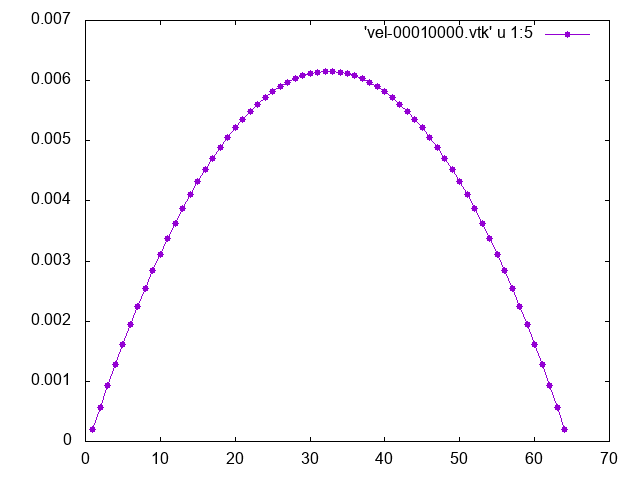
\includegraphics[width=0.6\linewidth]{velProf.png}
  \caption{The parabolic velocity profile of a simple fluid in a cavity after $10,000$ time-steps.}
  \label{fig:velocityProfile}
  \end{center}
\end{figure}

\subsection{Test 2: Spinodal Decomposition of a Binary Fluid}

This section outlines the second example, the spinodal decomposition of a binary fluid in 
three-dimensions.
The example describes the post-processing procedure for this system and a brief guide to 
the visualisation of a 3D system using ParaView.
As in the previous example, the code should be compiled in parallel and the executable 
\texttt{Ludwig.exe} should be copied into your working directory.

\begin{enumerate}
\item Copy the input file \texttt{input} located in the directory 
\texttt{/docs/tutorial/test2} 
to your working directory. This input file contains the parameters required for this run. 
\item Run the code in your working directory by issuing the command:
\begin{lstlisting}
$ mpirun -np 8 ./Ludwig.exe input
\end{lstlisting}
\item As before, you should now see statistics being reported on your standard output. But 
in this case two sets of output files are being created, one containing the velocity and 
the other compositional order parameter ($\phi$) data at each lattice point in the simulation. 
In this example, these data are in binary format.
\item The post-processing of the data requires again a compiled exectuable of \texttt{extract.c} in
\texttt{/util}, but this time with slightly different settings. 
Again, this requires the \texttt{Ludwig} code to be compiled in serial 
(see section \ref{configbuild}).
Specifically, set the flags for:
\begin{enumerate}
\item \texttt{input\_binary\_=1} \\ if the scalar order parameter and velocity data are in binary format (see 
flag in input file for \texttt{test2}),
\item \texttt{output\_binary\_=0} \\ as the output of the post-processing routines should be 
in ASCII format,
\item \texttt{output\_index=0} \\ as Cartesian lattice indices are not required, 
\item \texttt{output\_cmf=1} to produce data in column-major format, which is required for the correct 
visualisation with ParaView.
\end{enumerate}
\item Compile with 
\begin{lstlisting}
make extract
\end{lstlisting} 
and copy the executable \texttt{extract} into your working directory.
\item A python script \texttt{extract.py}
can be used for convenient post-processing of multiple raw data files and time steps.
 Edit \texttt{extract.py} and set:
\begin{enumerate}
\item \texttt{nstart=1000}, \texttt{nint=1000} and \texttt{nend=10000} to set the range and 
increments of the velocity data
to be processed.
\item \texttt{vel=1} for velocity post-processing, 
\item \texttt{phi=1} for $\phi$ post-processing,
\item The other flags should be set to zero. 
\end{enumerate}
\item Issue the command:
\begin{lstlisting}
$ python extract.py
\end{lstlisting}
\item You should now see files with the extension \texttt{.vtk} corresponding to the velocity 
and $\phi$ data ready to be visualised using ParaView.
\begin{enumerate}
\item In Paraview open the files containing the $\phi$ data.
\item Click on the group of files in the pipeline browser and apply a contour map using 
Filters/Common/Contour or in the tool bar: 

\begin{figure}[H]
\begin{center}
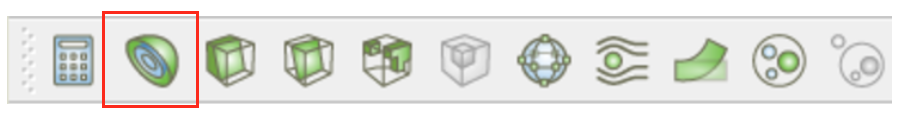
\includegraphics[width=0.8\linewidth]{contour.png}
  \caption{The contour button in the tool bar.}
  \label{fig:contour}
  \end{center}
\end{figure}

You should now see a three-dimensional rendering of the binary fluid.
\item Open the files containing the velocity data.
\item Click on the group of files in the pipeline browser and apply the glyph filter using 
Filters/Common/Glyph or in the tool bar: 

\begin{figure}[H]
\begin{center}
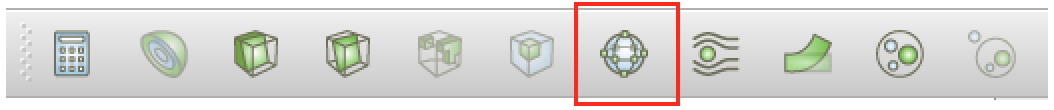
\includegraphics[width=0.8\linewidth]{glyph.png}
  \caption{The glyph button in the tool bar}
  \label{fig:glyph}
  \end{center}
\end{figure}

\item Change the colour code to GlyphVector Magnitude.
\item In the pipeline browser, you should see:

\begin{figure}[H]
\begin{center}
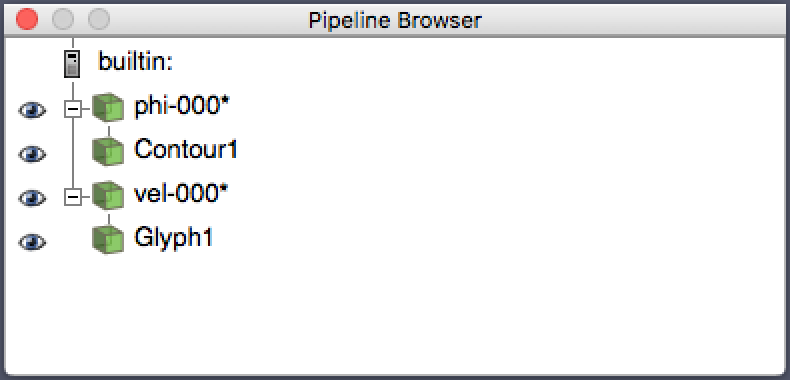
\includegraphics[width=0.6\linewidth]{pipeline.png}
  \caption{The complete pipline browser for the visualisation of spinodal decomposition.}
  \label{fig:pipeline}
  \end{center}
\end{figure}

A 3D visualisation of the system should also now be shown:

\begin{figure}[H]
\begin{center}
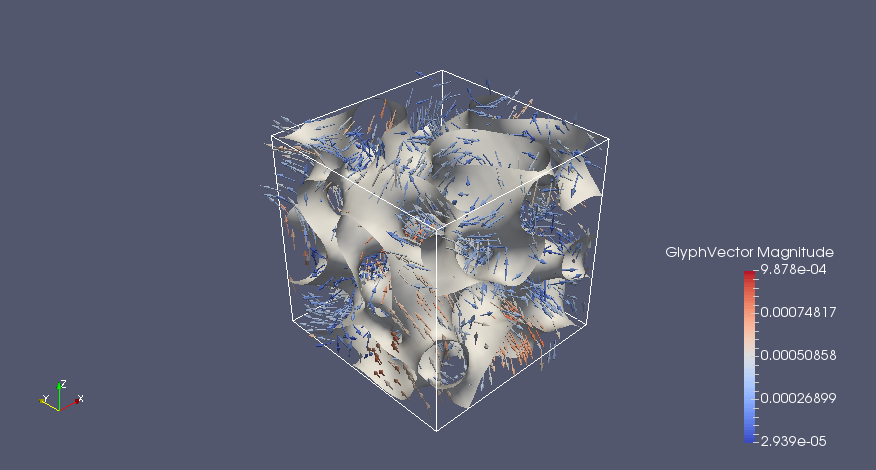
\includegraphics[width=0.6\linewidth]{system.png}
  \caption{A visualisation of a separating binary fluid using ParaView.}
  \label{fig:sysVisualisation}
  \end{center}
\end{figure}

\item You can move through different frames of the simulation with the arrow buttons:

\begin{figure}[H]
\begin{center}

\includegraphics[width=0.4\linewidth]{arrows.png}
  \caption{A visualisation of a separating binary fluid using ParaView.}
  \label{fig:changeFrame}
  \end{center}
\end{figure}

as you do this, you should see the coarsening of the binary fluid.

\item In the File menu you can save a screen shot of the visualisation or save the state of the system in order to reload the entire visualisation.
\end{enumerate}
\end{enumerate} 

\subsection{Test 3: Colloids Dispersed in a Liquid Crystalline Fluid}

For this third example, the system being used is a that of colloidal particles suspended in 
a liquid crystalline fluid.
The example illustrates the post-processing procedure for a colloidal system in addition to 
demonstrating the ways to visualise liquid crystals in ParaView. 
As before, the code should be compiled in parallel and the executable 
\texttt{Ludwig.exe} should be copied into your working directory.

\begin{enumerate}
\item Copy the input file \texttt{input} located in the directory 
\texttt{/docs/tutorial/test3} to your working directory. We see in this input file that 
there are many more parameters 
than in the previous examples. Specifically, we note that \texttt{colloid\_cell\_min} 
must be set if colloids are present and must be at least $2r + \delta$ where $r$ is colloid 
radius and $\delta$ - here set to 0.5 - catches any colloid-colloid interactions. This is shown for our example - where this value is set to 8.0 - in Fig. \ref{fig:colloid_int}.

 \begin{figure}[H]
\begin{center}
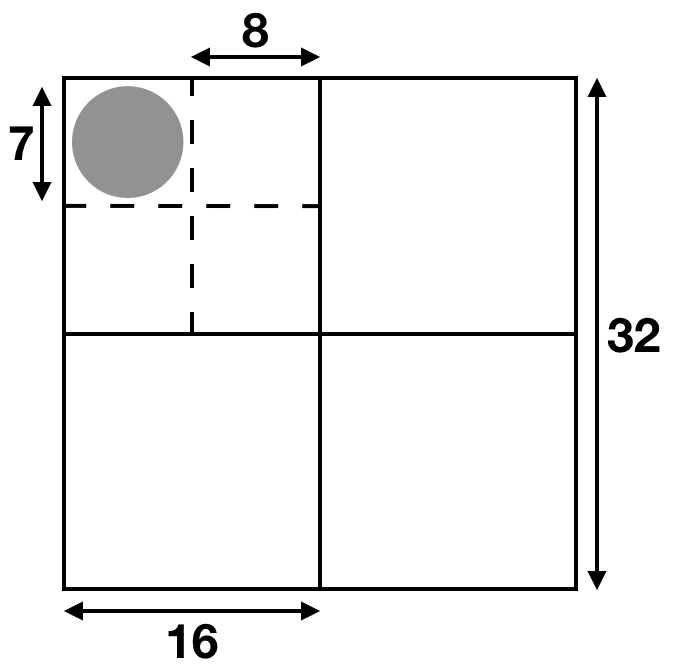
\includegraphics[width=0.5\linewidth]{colloidInit.png}
  \caption{A diagrammatic representation of a colloid in a 32$^3$ system showing that the value, \texttt{colloid\_cell\_min} must be set such that it can contain the entire colloid plus colloid-colloid interactions.}
  \label{fig:colloid_int}
  \end{center}
\end{figure}

\item The following steps outline the preliminary stages required in order to initialise the colloidal system and for the visualisation of colloids. Firstly, and as before, compile the \texttt{Ludwig} code in serial (see section \ref{configbuild}) and go to the directory \texttt{ludwig/util}. There you should see the files \texttt{colloid\_init.c} and \texttt{extract\_colloid.c}. These are the files required for the initialisation and post-processing of colloids, respectively.
\item In the file, \texttt{colloid\_init.c} set the flags for:
\begin{enumerate}
\item \texttt{NMC = 0},
\item \texttt{periodic[3] = {1,1,1}} \\ for our fully periodic system,
\item \texttt{file\_format=ASCII} \\ resulting in ASCII output,
\item \texttt{a0 = 3.5} \\ which sets the radius of the colloids,
\item \texttt{ah = 3.5} \\ which sets the hydrodynamic radius of the colloid,
\item \texttt{vf = 0.02} \\ this sets the volume fraction of colloids to 2\%, for our system of size 32$^2$ with colloids of radius 3.5, this will result in 3 colloids,
\item \texttt{dh = 0.5} \\ to set the grace distance for interactions (note that this means that one colloid plus this distance is less than \texttt{colloid\_cell\_min} which was set in the input file.
\end{enumerate}
\item Now issue: \\
\begin{lstlisting}
$ make colloid_init
$ ./colloid_init
\end{lstlisting}
this produces a file \texttt{config.cds.init.001-001}, which you have to copy into your working directory.
\item In the file, \texttt{extract\_colloids.c} set:
\begin{enumerate}
\item The system size, \texttt{NX},  \texttt{NY},  \texttt{NZ} all = 32,
\item \texttt{iread\_ascii = 1} \\ since the output is in ASCII,
\item \texttt{cds\_with\_v  = 1} \\ which will output the positions and velocity data of the colloids,
\end{enumerate}
\item Now issue: \\
\begin{lstlisting}
$ make extract_colloids
\end{lstlisting}
and copy the executable \texttt{extract\_colloids} into your working directory.
\item For the post-processing of this system, in \texttt{extract.c}, set:
\begin{enumerate}
\item \texttt{input\_binary\_  = 1} \\ due to binary output from code,
\item \texttt{output\_binary\_ = 0} \\ for output to be visualised in ASCII,
\end{enumerate}
compile in the usual manner and copy the post-processing executable \texttt{extract} and 
the script \texttt{extract.py} as well into your working directory. 
\item In \texttt{extract.py},
\begin{enumerate}
\item \texttt{vel = 1}, \\ to visualise the velocity field,
\item \texttt{q = 1}, \\ since there are liquid crystals present,
\item \texttt{colcds = 0} and 
\item \texttt{colcdsvel = 1} so that the colloid position and velocity data are both available.
\end{enumerate}

\item Next, run the code in your working directory by issuing the command:
\begin{lstlisting}
$ mpirun -np 8 ./Ludwig.exe input
\end{lstlisting}

\item Run the post-processing routine as before using the python script. 
\texttt{.csv} files with the colloid data should 
be seen in addition to the \texttt{.vtk} files for the velocity, order parameter and director field.
\item The system can now be visualised, again using ParaView:
\begin{enumerate}
\item The liquid crystal, scalar order parameter can be visualised by opening the files: 
\texttt{lcs-XXXXXXXX.vtk} and applying the `contour' filter. By setting a threshold 
minimum $1 \times 10^{-4}$ the order parameter in the colloids can be ignored, this can be done using the tool bar:

\begin{figure}[H]
\begin{center}
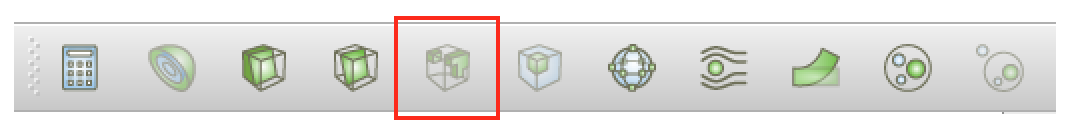
\includegraphics[width=0.8\linewidth]{thresh.png}
  \caption{The threshold button in the tool bar.}
  \label{fig:thresh}
  \end{center}
\end{figure}

\item For the director field open the \texttt{lcd-XXXXXXXX.vtk} and apply the `glyphvector' filter. In this case, change the glyph 
type from `arrow' to `line' and scale the colour of the lines by the $x$-component of the 
vector.
\item The velocity field can be visualised using arrows as before with the `glyphvector' filter.
\item To visualise the colloids, open the files \texttt{col-cdsXXXXXXXX.csv}. This will open 
a table, which can be closed. Next apply the filter `Table to Points' found in 
Filters/Alphabetical/Table to Points and set the X, Y and Z Columns in the `Properties' tab 
below the Pipeline Browser to be the $x$, $y$ and $z$-coordinates in the table via the 
drop down menus:

\begin{figure}[H]
\begin{center}
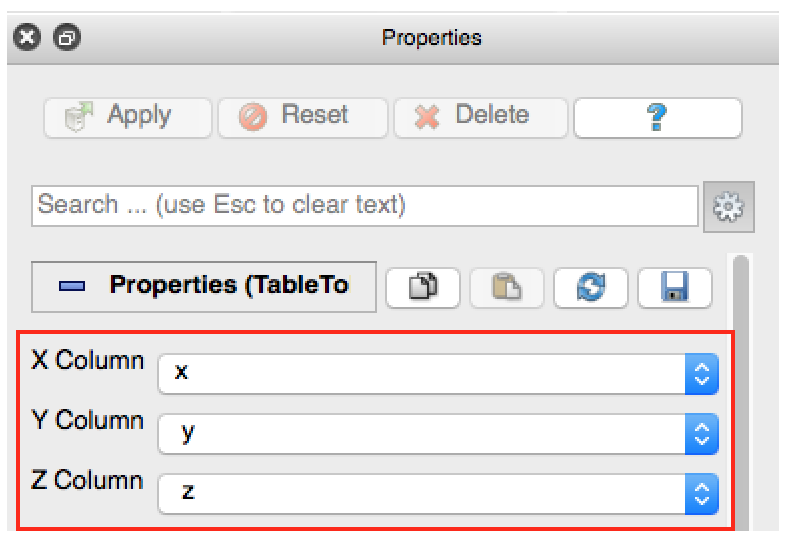
\includegraphics[width=0.5\linewidth]{colloidCoords.png}
  \caption{Setting the coordinates of the colloid locations in the properties tab.}
  \label{fig:collCoords}
  \end{center}
\end{figure}

 You should now see points in the render window at the location of the centres of each of the colloids.
\item To fully visualise the colloids, apply the `glyphvector' filter and set glyph type to 
`sphere.' In the properties tab, set the radius to 3.5, scale mode `off' and scale factor to 
1.0 in the properties. In order to access these settings, you will need to click the `cog' icon shown here:

\begin{figure}[H]
\begin{center}
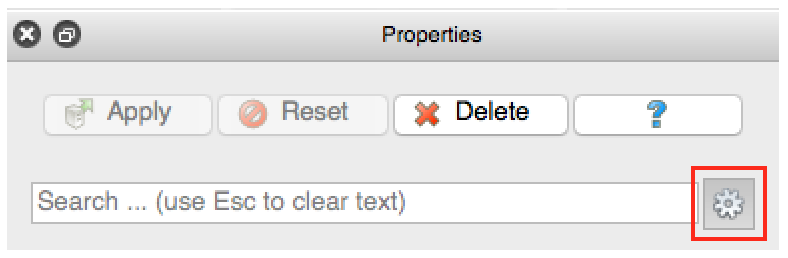
\includegraphics[width=0.5\linewidth]{cog.png}
  \caption{Location of the `cog' icon in the properties tab.}
  \label{fig:cog}
  \end{center}
\end{figure}

\item Next, glyph mode must be set to `all points' and you should set the colour of teh spheres to `Solid Color'. Finally, you can increase the resolution of the spheres by increasing the `Theta Resolution' and `Phi Resolution' quantities.
\item In the pipeline browser, should now see: 

\begin{figure}[H]
\begin{center}
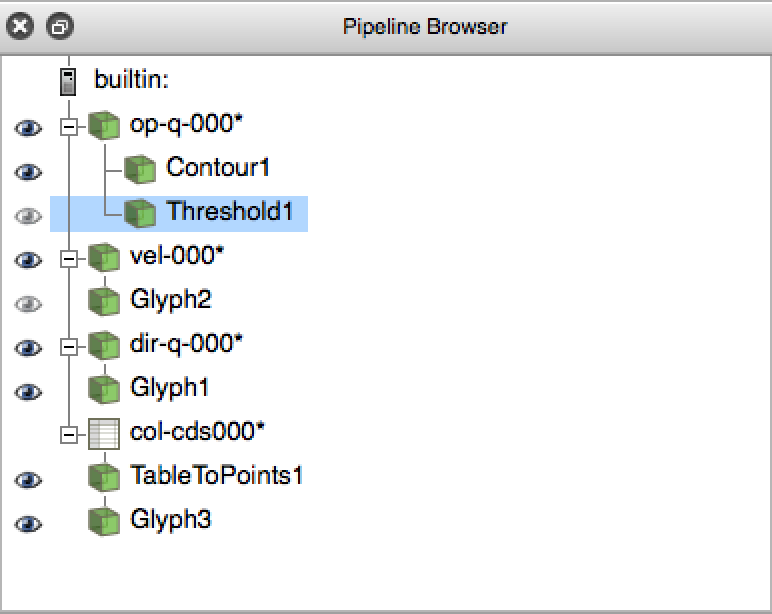
\includegraphics[width=0.6\linewidth]{colloidsPipeline.png}
  \caption{The pipeline browser for the colloidal suspension in liquid crystals.}
  \label{fig:collPipe}
  \end{center}
\end{figure}

The 3D visualisation of this system should appear as:

\begin{figure}[H]
\begin{center}
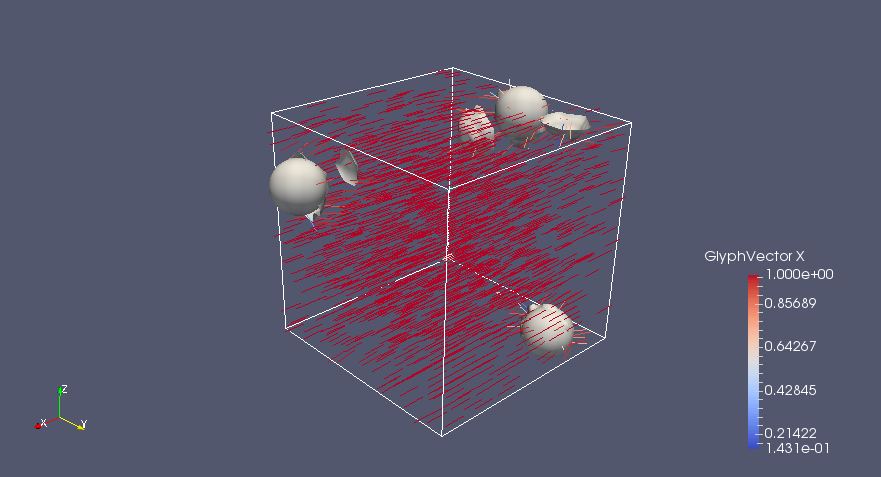
\includegraphics[width=0.6\linewidth]{colloidSystem.png}
  \caption{The visualisation of the colloidal suspension in liquid crystals.}
  \label{fig:collVis}
  \end{center}
\end{figure}


\end{enumerate}
\end{enumerate}

%\clearpage
%\vfill\pagebreak
%%%%%%%%%%%%%%%%%%%%%%%%%%%%%%%%%%%%%%%%%%%%%%%%%%%%%%%%%%%%%%%%%%%%%%%%%%%%
%
%  references.tex
%
%  Bibliography
%
%  $Id$
%
%  Edinburgh Soft Matter and Statistical Physics Group and
%  Edinburgh Parallel Computing Centre
%
%  Kevin Stratford (kevin@epcc.ed.ac.uk)
%  (c) 2011 The University of Edinburgh
%
%%%%%%%%%%%%%%%%%%%%%%%%%%%%%%%%%%%%%%%%%%%%%%%%%%%%%%%%%%%%%%%%%%%%%%%%%%%

\vfill
\pagebreak

\addcontentsline{toc}{section}{References}

\bibliographystyle{plain}
\begin{thebibliography}{99}

\bibitem{adhikari_desplat}
Adhikari, R. J.-C. Desplat, and K. Stratford,
Sliding periodic boundary conditions for lattice Boltzmann and lattice
kinetic equations,
\texttt{arXiv:cond-mat/0503175v1} (2005).

\bibitem{adhikari2005}
Adhikari, R., K. Stratford. M.E. Cates, and A.J. Wagner,
Fluctuating Lattice Boltzmann,
\textit{Europhys. Lett.}, \textbf{71}, 473 2005.

\bibitem{ald98}
Aidun, C.K., Y. Lu, and E.-J. Ding,
Direct analysis of particulate suspensions with inertia using the
discrete Boltzmann equation,
\textit{J. Fluid Mech.}, \textbf{373}, 287, 1998.

\bibitem{batchelor}
G.K. Batchelor
\textit{An Introduction to Fluid Mechanics},
Cambridge University Press (1967).

\bibitem{blake}
J.R. Blake, A spherical envelope approach to ciliary propusion,
\textit{J. Fluid Mech.}, \textbf{46}, 199, 1971.

\bibitem{cates_scaling}
M. E. Cates, J.-C. Desplat, P. Stansell, A.J. Wagner, K. Stratford,
R. Adhikari, and I. Pagonabarraga,
Physical and Computational Scaling Issues in Lattice Boltzmann
Simulations of Binary Fluid Mixtures,
\textit{Phil. Trans. Roy. Soc. A}, \textbf{363}, 1917 (2005). 

\bibitem{chunladd}
B. Chun and A.J.C. Ladd,
Interpolated boundary condition for lattice Boltzmann simulations in
narrow gaps,
\textit{Phys. Rev. E}, \textbf{75}, 066705, 2007.

\bibitem{cj98}
Cichocki, B., and R.B. Jones,
Image representation of a spherical particle near a hard wall,
\textit{Physica A}, \textbf{258}, 273, 1998.

\bibitem{chang}
C.-H. Chang and E.I. Franses,
Adsorption dynamics of surfactants at the air/water interface:
a critical review of mathematical models, data, and mechanisms,
\textit{Colloids and Surfaces A}, \textbf{100} 1, 1995.

\bibitem{cpc}
Desplat, J.-C., I. Pagonabarraga, and P. Bladon,
LUDWIG: A parallel lattice-Boltzmann code for complex fluids.
\textit{Comput. Phys. Comms.}, \textbf{134}, 273, 2001.

\bibitem{diamant}
H. Diamant and D. Andelman,
Kinetics of surfactant adsorption at fluid/fluid
interfaces: non-ionic surfactants,
\textit{Europhys. Lett.} \textbf{34}, 575 (1996).

\bibitem{diamant96}
H. Diamant and D. Andelman,
Kinetics of surfactant adsorption at fluid-fluid interfaces,
\textit{J. Phys. Chem.}, \textbf{100} 13732, 1996.

\bibitem{fournier2005}
J.-B. Fournier and P. Galatola,
Modeling planar degenerate wetting and anchoring in nematic liquid
crystals,
\textit{Europhys. Lett.}, \textbf{72} 403--409 (2005).

\bibitem{eastoe}
J. Eastoe and J.S. Dalton,
Dynamic surface tension and adsorption mechanims of surfactants
at the air-water interface,
\textit{Advances in Colloid and Interface Science}, \textbf{85}
13, 2000.

\bibitem{ginzburg}
I. Ginzburg and D. d'Humi\`eres,
Multireflection boundary conditions for lattice Boltzmann models,
\textit{Phys. Rev. E}, \textbf{68}, 066614, 2003.

\bibitem{h59}
Hasimoto, H., On the periodic fundamental solutions of the Stokes
equation and their application to viscous flow past a cubic array
of spheres.
\textit{J. Fluid Mech.}, \textbf{5}, 317.

\bibitem{heemels}
Heemels, M.W., M.H.J. Hagen, and C.P. Lowe, Simulating solid colloidal
particles using the lattice-Boltzmann method,
\textit{J. Comp. Phys.}, \textbf{164}, 48, 2000.

\bibitem{ieee-208}
IEEE Standard 208-2005, IEEE Standard for Software Configuration Management
Plans. See \texttt{http://ieeexplore.ieee.org/xpl/standards.jsp}
(accessed 2011).

\bibitem{jo84}
Jeffrey, D.J., and Y. Onishi,
Calculation of the resistance and mobility functions for the two
unequal rigid spheres in low-Reynolds-number flow,
\textit{J. Fluid Mech.}, \textbf{139}, 261, 1984.

\bibitem{viv}
Kendon, V.M., M.E. Cates, I. Pagonabarraga, J.-C. Desplat, and
P. Bladon,
Inertial effects in three dimensional spinodal decomposition of
a symmetric binary fluid mixture: A lattice Boltzmann study,
\textit{J. Fluid Mech.}, \textbf{440}, 147 (2001).

\bibitem{l94a}
Ladd, A.J.C., Numerical simulations of particulate suspensions
via a discretised Boltzmann equation. Part 1. Theoretical foundation,
\textit{J. Fluid. Mech.}, \textbf{271}, 285, 1994.

\bibitem{l94b}
Ladd, A.J.C., Numerical simulations of particulate suspensions
via a discretised Boltzmann equation. Part 2. Numerical results,
\textit{J. Fluid. Mech.}, \textbf{271}, 311, 1994.

\bibitem{l96a}
Ladd, A.J.C., Sedimentation of homogenous suspensions of non-Brownian
spheres,
\textit{Phys. Fluids}, \textbf{9}, 491. 1996.

\bibitem{l96b}
Ladd, A.J.C., Hydrodynamic screening in sedimentating suspensions
of non-Brownian spheres,
\textit{Phys. Rev. Lett.}, \textbf{76}, 1392, 1996.

\bibitem{lv01}
Ladd, A.J.C., and R. Verberg,
Lattice-Boltzmann simulations of particle-fluid suspensions,
\textit{J. Stat. Phys.}, \textbf{104}, 1191, 2001.

\bibitem{lipanmiller}
H. Li, C. Pan, and C.T. Miller,
Pore-scale investigation of viscous coupling effects for two-phase
flow in porous media,
\textit{Phys. Rev. E}, \textbf{72}, 026705, 2005.

\bibitem{lighthill}
M.J. Lighthill,
On the squirming motion of nearly spherical deformable bodies through
liquid at very small Reynolds numbers,
\textit{Comm. Pure Appl. Math.}, \textbf{5}, 109, 1952.

\bibitem{isaac}
I. Llopis Fust\'e,
\textit{Hydrodynamic cooperativity in micro-swimmer suspensions},
Ph.D. Thesis, University of Barcelona, 2008.

\bibitem{mpi-standard}
Message Passing Interface Forum. MPI: A Message Passing Interface Standard
Version 1.3 (2008).

\bibitem{nguyen-ladd2002}
Nguyen, N.-Q., and A.J.C. Ladd, Lubrication corrections for
lattice-Boltzmann simulations of particle suspensions,
\textit{Phys. Rev. E}, \textbf{66}, 046708, 2002.

\bibitem{papanastasiou}
T. paapnastasiou, G. Georgiou, and A. Alexandrou,
\textit{Viscous Fluid Flow},
CRC Press, Boca Raton, Florida, 2000.

\bibitem{paraview}
Paraview. See \texttt{http://www.paraview.org/}. Accessed 2011.

\bibitem{r95}
Rapaport, D.C., \textit{The Art of Molecular Dynamics Simulation},
Cambridge University Press, 1995.

\bibitem{succi}
S. Succi, \textit{The lattice Boltzmann equation and beyond},
Oxford University Press, Oxford, 2001.

\bibitem{edo1}
M. Venuroli and E.S. Boek,
Two-dimensional lattice-Boltzmann simulations of single phase
flow in a pseudo two-dimensional micromodel,
\textit{Physica A}, \textbf{362}, 23, 2006.

\bibitem{vandergraaf}
R.G.M. van der Sman and S. van der Graaf,
Diffuse interface model of surfactant adsorption onto flat and
droplet interfaces,
\textit{Rheol. Acta} \textbf{46} 3 (2006).

\bibitem{theissengompper}
O. Theissen and G. Gompper,
Lattice Boltzmann study of spontaneous emulsification,
\textit{Eur. Phys. J. B}, \textbf{11} 91 (1999).

\bibitem{wardtordai}
A.F.H. Ward and L. Tordai,
\textit{J. Chem. Phys.} \textbf{14} 453, 1946.

\bibitem{skarabot}
M. Skarabot, M. Ravnik, S. Zumer, U. Tkalec, I. Poberaj, D. Babic, N. Osterman and I. Musevic,
\textit{Phys. Rev. E} \textbf{76}, 051406 (2007).

\bibitem{wright}
D.C. Wright and N.D. Mermin,
\textit{Rev. Mod. Phys.} \textbf{61}, 385 (1989).

\bibitem{Lyklema} J. Lyklema {\em Fundamentals of Interface and Colloid Science} Academic Press     (1995).
\bibitem{Mafe} S. Maf\'e, J.A. Manzanares, J. Pellicer, {\textit J. Electroanal. Chem.} {\textbf 241}, 5    7-77 (1988).
\bibitem{Capuani} F. Capuani, I. Pagonabarraga, D. Frenkel, {\textit J. Chem. Phys.} {\textbf 121}, 973-    986 (2004).
\bibitem{Rotenberg} B. Rotenberg, I. Pagonabarraga, D. Frenkel, {\textit Farad. Discuss.} {\textbf 144},     223-243 (2010).
\bibitem{Landau-ED} L.D. Landau, E.M. Lifshitz, {\textit Electrodynamics of Continuous Media}, \S 15    , 2nd ed., Pergamon Press, Oxford, UK (1984).
\bibitem{Melcher} J.R. Melcher, {\textit Continuum Electromechanics}, \S 3.10, MIT Press, Cambridge,     MA, USA (1981).\\
downloadable from:\\
\url{http://ocw.mit.edu/ans7870/resources/melcher/resized/cem_811.pdf}
\bibitem{Landau-EL} L.D. Landau, E.M. Lifshitz, {\textit Theory of Elasticity}, \S 3 \& \S 16, 3rd e    d., Butterworth-Heinemann, Oxford, UK (1986).



\end{thebibliography}




\end{document}
